\documentclass[a4paper,11pt]{article}
\usepackage[T1]{fontenc}
\usepackage{inputenc}
\usepackage{amsfonts}
\usepackage{graphicx}
\usepackage{bm}
\usepackage{varioref}
\usepackage[english]{babel}
\usepackage{hyperref}
\usepackage{tikz}
\usetikzlibrary{arrows,decorations.pathmorphing,backgrounds,positioning,fit,petri}
\usepackage{enumitem}
\usepackage{newclude}
\newcommand{\field} [1] {\mathbb{#1}}
\begin{document}

\begin{titlepage}
\centering \parindent=0pt
\newcommand{\HRule}{\rule{\textwidth}{1mm}}
\vspace*{\stretch{1}} \HRule\\[1cm]\Huge\bfseries
Semester Project\\\emph{Slice of Pie}\\[0.7cm]
\HRule\\[4cm]  \large Group 8
\\Jacob Stenum Czepluch (jstc@itu.dk), \\Niels Roesen Abildgaard (nroe@itu.dk), \\Niclas Tollstorff (nben@itu.dk), \\Sigurt Bladt Dinesen (sidi@itu.dk), \\Michael Storgaard (mmun@itu.dk)\\
\vspace*{\stretch{2}} \normalsize %
\begin{flushleft}
Semester Project\\
Bachelor in Software Development\\
IT-University of Copenhagen\\
Jacob Bardram (bardram@itu.dk)\\
Dario Pacino (dpacino@itu.dk) \\
December 17, 2012 \end{flushleft}
\end{titlepage}

\tableofcontents
\pagebreak

% This is how a section is created.
\pagebreak
\section{Introduction}
\include*{Introduction/introduction}

\pagebreak
\section{User manual}
\include*{User_manual/main}

% This is how a subsection is created.
\subsection{Noob manual}
% Not really sure what this does or if neccessary. \label{sec:User manual}
\include*{User_manual/noob}

\pagebreak
\section{Software Analysis}
\include*{Software_analysis/main}

\subsection{Use Cases}
\include*{Software_analysis/use_cases}

\subsection{Domain Model}
\include*{Software_analysis/domain_model}

\subsection{System Sequence Diagrams}
\include*{Software_analysis/ssd}

\subsection{FURPS+}
\include*{Software_analysis/furps}

\pagebreak
\section{Software Design}
\include*{Software_design/main}

\subsection{Class Diagrams}
\include*{Software_design/class_diagrams}

\subsection{Interaction Diagrams}
\include*{Software_design/interaction_diagrams}

\subsection{Design Patterns}
\include*{Software_design/design_patterns}
\subsubsection{Asynchronous Calls through APM}
\label{sec:APM}

For a desktop UI to be responsive, it is important that heavy loads are moved away from the UI thread.
There are several possible ways of doing this: threading, abstracting to using tasks, or asynchronous
methods. To reduce the amount of boilerplate code in the UI layer, the responsibility for delegating
to threads was moved to the controller.

The \emph{Asynchronous Programming Model}\cite{msdnAPMdoc} (abbreviated \emph{APM}) allows for easy,
asynchronous calls to heavy-duty methods at a nice level of abstraction, substantially simplifying UI
programming. The support for callbacks lets the UI react as soon as a job finishes, without having to
continuously poll the model (although this approach is also possible through the APM).

There are no built-in building blocks for implementing the APM in C\#, however the MSDN Magazine\cite{richtermsdn0307}
brought an article by Jeffrey Richter guiding the process. Based on these ideas, building custom APM becomes easier and
this is the way we chose to go with the controller.

The Asynchronous Programming Model can be used to wrap normal, blocking methods (from here on referred to as
the \emph{inner method}) in an asynchronous context, while still allowing the caller to react on results
returned by the method through a callback delegate.

All APM calls consist of two methods, one prefixed with \emph{Begin} and another with \emph{End} (ie.
when wrapping inner method \emph{GetProjects(userMail)}, the resulting methods would be \emph{BeingGetProjects}
and \emph{EndGetProjects}). The Begin-method is passed not only the arguments required by the inner method call
(ie. \emph{userMail}) but also a callback-delegate and a state-object.

Calling the Begin-method returns almost instantaneously; under the covers, it commandeers a different thread
on which to execute the inner method.

\begin{figure}[hbt]
    \begin{verbatim}
    
    
public IAsyncResult BeginGetProjects(string userMail,
            AsyncCallback callback, object state);\end{verbatim}
    \caption{Method declaration for the BeginGetProjects method}
    \label{fig:begingetprojectscode}
\end{figure}

The state object is less important for our case, as it is not actually used in our implementation. It can be used
to pass arbitrary information to the callback.

The callback is a delegate (\emph{AsyncCallback} from the \emph{System} namespace\footnote{See more details about this delegate on MSDN: http://msdn.microsoft.com/en-us/library/system.asynccallback.aspx})
taking a single parameter of type \emph{IAsyncResult}, which will be the same object as the one
returned by \emph{BeginGetProjects} (Figure \ref{fig:begingetprojectscode}) and a void return type.
In the callback, the first method call should be to the End-method with the IAsyncResult
as a parameter. This call blocks until the inner method returns and then passes the result along.

Note that the End-method may also be called outside of the callback. This would result in the code
blocking until the inner method returns, and as such would not be desirable in a User Interface.

Additionally, when using this kind of asynchronous calls, it is important to note that the callback
is executed on a different thread (in our case a thread in the ThreadPool) from the one the Begin-method
was called on. As such, one should keep an eye out for the synchronization context when updating UI
elements.\cite[p.~622]{Griffiths2010}

\begin{figure}[hbt]
    \begin{verbatim}
    
    
SynchronizationContext syncContext = SynchronizationContext.Current;

controller.BeginGetProjects("dummy@email.com", (asyncResult) => {
    syncContext.Post(RefreshUI(controller.EndGetProjects(asyncResult)))
}, null);\end{verbatim}
\caption{Correct usage of APM in a user interface-context, taking synchronization contexts into account; paraphrased over code in MainWindow.xaml.cs of the \SOP{} project.}
    \label{fig:apmuserinterfacecode}
\end{figure}

\paragraph{Implementation}

The \SOP{} implementation of APM is influenced heavily by Richter's article, having a couple of
implementations of the IAsyncResult interface. These implementations either have a void return type
or a generic one and take a number (0 - 3) parameters, also generically typed.

As our implementation focuses on reusability, these generic classes were built to accomodate any
unforeseeable method that we may wish to wrap in this pattern.

In an additional attempt to reduce code duplication construction of a factory for automatically
generating these wrapper-methods was begun, however it was never fully implemented.

\paragraph{Task-Parallel Library}

Another advantage with the APM pattern is that it is nicely supported by the \emph{Task Parallel Library}\cite[p.~656]{Griffiths2010}
(TPL), allowing for them to be used in a simple interface with great concurrency and error-handling support, as well as chaining up
several methods in continuation.


\pagebreak
\section{Software Architecture Documentation}
\include*{Software_architecture/main}

\subsection{Architecture Analysis}
\include*{Software_architecture/architecture_analysis}

\subsection{Factor Tables}
\include*{Software_architecture/factor_tables}

\subsection{Logical Views}
\include*{Software_architecture/logical_views}

\subsection{Deployment Views}
\include*{Software_architecture/deployment_views}

\pagebreak
\section{SCRUM}
\include*{SCRUM/main}

\subsection{Distribution of SCRUM roles}
\include*{SCRUM/distribution_of_scrum_roles}

\subsection{The Product Backlog}
\include*{SCRUM/the_product_backlog}

\subsubsection{Definition of Done}
\include*{SCRUM/definition_of_done}

\subsection{The Sprint cycle}
\include*{SCRUM/the_sprint_cycle}

\pagebreak
\section{Testing}
\include*{Testing/main}

\subsection{Test Strategy}
\include*{Testing/strategy}

\subsection{Test Results}
\include*{Testing/results}

\pagebreak
\section{Discussion}
\include*{Discussion/main}

\pagebreak
\section{Reflection}
\include*{Reflection/main}

\pagebreak
\section{Conclusion}
\include*{Conclusion/main}

\pagebreak
\section{User manual}
\subsubsection{Projects}
Projects are the primary container entity in the program and can contain folders or documents, but not other projects.
Projects are the root-elements in Slice of Pie, and can be shared with other users.

\subsubsection{Folders}
Folders are a container entity in the program, which can contain folders or documents. Folders has to be created inside either a project or another folder.

\subsubsection{Documents}
Documents are the primary entity in the program, as it holds all textual content.

\subsection{Local client}

The local client is mostly working offline, but some features (like sharing projects, synchronizing and retrieving document history) require an
internet connection to be established. Changes are only applied globally, when the data is synchronized.

\begin{figure}[htb]
	\centering
	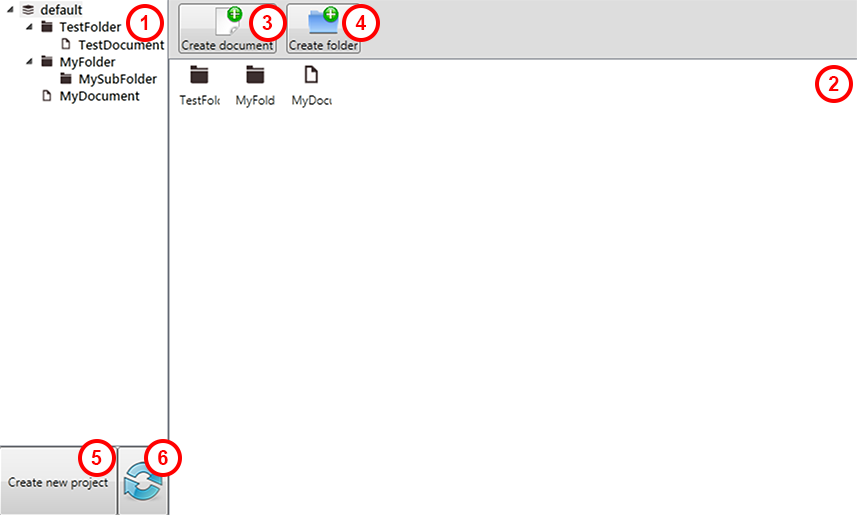
\includegraphics[width=1\textwidth]{User_manual/graphics/local.png}
	\caption{Screenshot of the local client}
	\label{fig:manual-local}
\end{figure}

You are not logged in, when you are using the local client, but it does require authentication whenever you wish to interact with online data.

\subsubsection{Projects}

	\paragraph{Create project}
	To create a new project, click the Create new project button (5 in figure~\ref{fig:manual-local}) and enter the desired name in the pop-up window. You can now find your new project in the explorer (1 in figure~\ref{fig:manual-local}).

	\paragraph{Share project}
	In order to share a project in the local client, you need to have an internet connection established and your data
    has to be synchronized at some point before, meaning you do not have to have an up-to-date project, folder or
    document, but the project has to exist online. When these requirements are fulfilled, you can right-click a project
    in the explorer (1 in figure~\ref{fig:manual-local}) and click Share project. This will open a pop-up window with
    a text field, which can handle both single email addresses or comma-separated lists of email addresses.

	\paragraph{Remove project}
	To remove a project, right-click the project in the explorer (1 in figure~\ref{fig:manual-local}) and click Remove project. Be aware that all subitems (folders and documents) will also be removed.

	\paragraph{Synchronize}
	In order to synchronize your data, you need to have an internet connection established. When that requirement is fulfilled, you can synchronize your data, by clicking the synchronize button (6 in figure~\ref{fig:manual-local}) and entering your account information in the pop-up window. If the user does not exist, a new one will be created with the desired account information. All data will then be synchronized, which can take several moments.

\subsubsection{Folders}

	\paragraph{Create folder}
	To create a new folder, click the Create folder button (4 in figure~\ref{fig:manual-local}) or right-click a project or folder in the explorer (1 in figure~\ref{fig:manual-local}) and click Create folder. Then enter the desired name in the pop-up window. You can now find your new folder in the explorer as a subitem in the project or folder in which it was created.

	\paragraph{Remove folder}
	To remove a folder, right-click the folder in the explorer (1 in figure~\ref{fig:manual-local}) and click Remove folder.  Be aware that all subitems (folders and documents) will also be removed.

\subsubsection{Documents}

	\paragraph{Create document}
	To create a new document, click the Create document button (3 in figure~\ref{fig:manual-local}) or right-click a project or folder in the explorer (1 in figure~\ref{fig:manual-local}) and click Create document. Then enter the desired name in the pop-up window. You can now find your new document in the explorer as a subitem in the project or folder in which it was created.
	
	\paragraph{Edit document}
	To edit a document, click on the document in the explorer (1 in figure~\ref{fig:manual-local}). This will open the document with a large editing area (1 in figure~\ref{fig:manual-local-document}). When editing the document, you can use the \emph{HyperText Markup Language}\cite{w3cHTML} (HTML) to format your content. To save the document, simply click the Save document button (2 in figure~\ref{fig:manual-local-document}).
	
	\begin{figure}[htb]
		\centering
		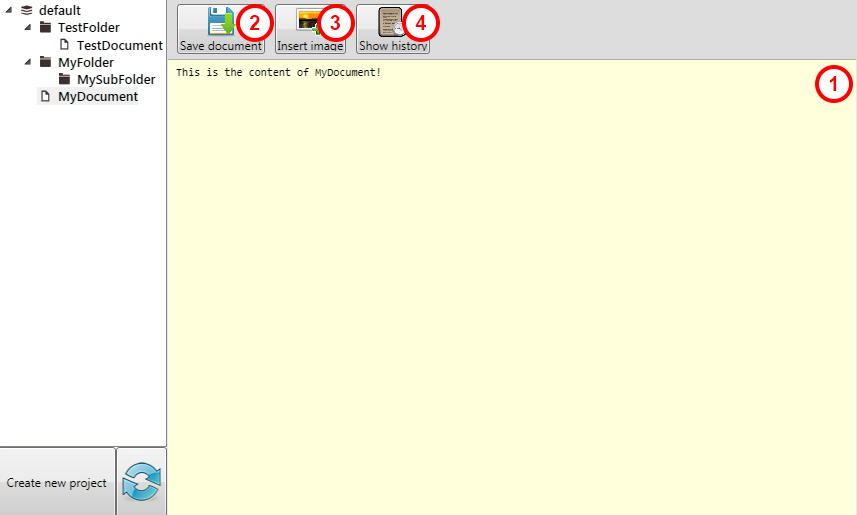
\includegraphics[width=1\textwidth]{User_manual/graphics/local-document.png}
		\caption{Screenshot of the document view in the local client}
		\label{fig:manual-local-document}
	\end{figure}
	
		\subparagraph{Insert image}
		To insert an image, click the Insert image button (3 in figure~\ref{fig:manual-local-document}) and enter the URL to the image in the pop-up window. This will insert an HTML image tag at the cursors position.
		
		\subparagraph{Show history}
		To view the revisions of a document, click the Show history button (4 in figure~\ref{fig:manual-local-document}). This will open a pop-up window with the most recent revision visible, while the rest of the history is available from the list in the left side of the window. You can copy the visible revision or part of it and paste it to your editor window.
	
	\paragraph{Remove document}
	To remove a document, right-click the folder in the explorer (1 in figure ~\ref{fig:manual-local}) and click Remove document. Be aware that all revisions will also be removed.


The web client requires a persistent internet connection and is making all changes in real-time. You are required to log in before using the web client. You will however create a new user, if you enter an email address not already known.

\begin{figure}[htb]
	\centering
	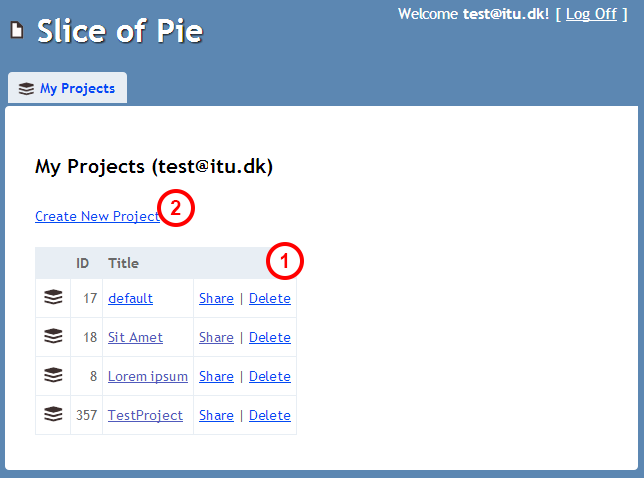
\includegraphics[width=1\textwidth]{User_manual/graphics/web.png}
	\caption{Screenshot of the web client}
	\label{fig:manual-web}
\end{figure}

\subsubsection{Projects}

	\paragraph{Create project}
	To create a new project, click the Create New Project button (2 in figure~\ref{fig:manual-web}) and enter the desired name on the new page. Your new project is now open and you can access an overview of folders and documents (like seen at 1 in figure~\ref{fig:manual-web}).

	\paragraph{Share project}
	To share a project, click the Share button in the overview (1 in figure~\ref{fig:manual-web}). This will lead you to a new page with a text area, which can handle both single email addresses or comma-separated email addresses.
	
	\paragraph{Remove project}
	To remove a project, click the Delete button in the overview (1 in figure~\ref{fig:manual-web}) and confirm. Be aware that all folders, subfolders and documents will also be removed.

\subsubsection{Folders}

	\paragraph{Create folder}
	In order to create a new folder, you have to be inside a project or another folder, from where you can click the Create New Folder button (like seen at 2 in figure~\ref{fig:manual-web}). Then enter the desired name on the new page. Your new folder is now open and you can access a list of folders and documents (like seen at 1 in figure~\ref{fig:manual-web}).

	\paragraph{Remove folder}
	To remove a folder, click the Delete button in the overview (1 in figure~\ref{fig:manual-web}) and confirm. Be aware that all subfolders and documents will also be removed.

\subsubsection{Documents}

	\paragraph{View document}
	To view a document, click the Show button in the overview (same location as the Share button in 1 in figure~\ref{fig:manual-web}). This will open a new page with the contents of the document formatted as HTML (1 in figure~\ref{fig:manual-web-document}).
	
	\begin{figure}[htb]
		\centering
		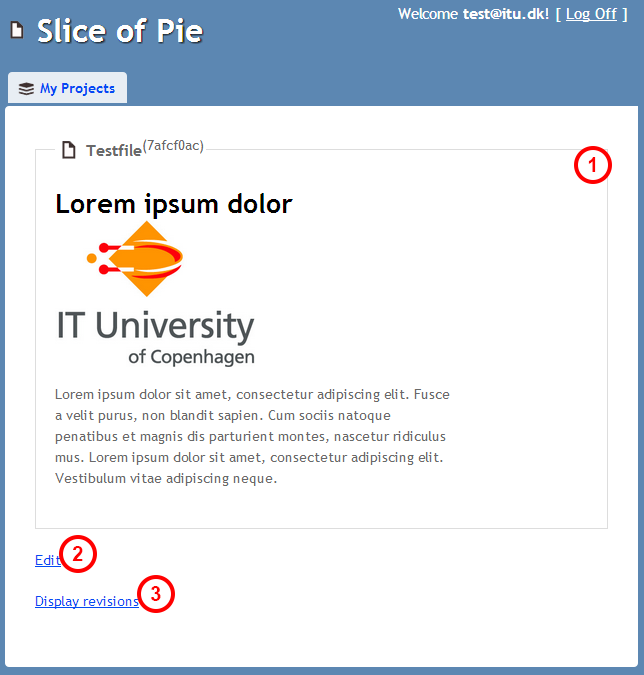
\includegraphics[width=1\textwidth]{User_manual/graphics/web-document.png}
		\caption{Screenshot of the document view in the web client}
		\label{fig:manual-web-document}
	\end{figure}
		
		\subparagraph{Show history}
		To view the revisions of a document, click the Display revisions button (3 in figure~\ref{fig:manual-web-document}) in the view of the document. This will show the revisions below the view of the document in a list with latest revision at the top.

	\paragraph{Create document}
	In order to create a new document, you have to be inside a project or another folder, from where you can click the Create New Document button (like seen at 2 in figure~\ref{fig:manual-web}). Then enter the desired name on the new page. Your new document is now open in editing mode.
	
	\paragraph{Edit document}
	To edit a document, either click on the document name in the overview (1 in figure~\ref{fig:manual-web}) or click the Edit button (2 in figure~\ref{fig:manual-web-document}) in the view of the document. When editing the the document, you can use the \emph{HyperText markup language}\cite{w3cHTML} (HTML) to format your content. To save the document, click the Edit button below the text box.
	
	\paragraph{Remove document}
	To remove a document, click the Delete button in the overview (1 in figure ~\ref{fig:manual-web}) and confirm. Be aware that all revisions will also be removed.


\pagebreak
\appendix
% include appendices here

\end{document}
